%\documentclass{article}
\documentclass{IEEEtran}
\usepackage[utf8]{inputenc}

\title{Week2 Journal.}
\author{Theodore Longtchi}
\date{September 2019}

\usepackage{natbib}
\usepackage{graphicx}

\begin{document}

\maketitle

\section{The Learning Process}
Although I initially registered to take this course – CS 6000 – because it is a core requirement for my PhD degree in Engineering with concentration in Security, the past two class sessions have demonstrated the need for the class for regular research students like myself. Before these classes, I would at least scan papers to chose the ones that were interesting to further read them. The problem was that I usually did not finish the browsing due to the fact that I spent too much time going through the list of papers in the first round. Initially, I would trash a paper just by its title, and I believe that caused me to miss reading papers with hidden or not so-much explicit titles. Sometimes even if I had to browse, and it was not sounding like the exact thing that I wanted, I would just thrash the paper. I have learned to at least give each paper a chance by taking at least a minute to browse.  

The different stages of reading a paper is another major thing I have learned at this point in time in this course. Usually, I would spent the first time trying to understand the content of a paper, although I would leave the Math for later. I have learned to just get a high level picture of what the paper is all about without getting into any further details. I also never really verified the references, because I believe the authors would not reference something they did not use, or reference something they did not understand. So I usually just assume all the references were worth referencing. It did not occur to me that even papers that are published in highly accredited journals or conferences may have that flaw or wrong referencing or misunderstood referencing.    

The intention I had when going through a paper was almost like that of going through a textbook. I felt like it was established facts that had gone through peer review, and all I needed to do was to learn the concept or whatever the paper was aiming to do. I really never thought of questioning things like methodology or evaluating the paper's claims. To me, it was like an established fact, and all I had to do was to learn it. I now understand that, the fact that one questions those aspects of the paper also helps in building one's own capacity of critical thinking, which results to learning something concrete.

Another striking thing is the sweeping generalization, bias, prejudice. Maybe I could have been able to point some of these things, but it was not so clear in my mind the way it is clear now. I know that I have to read a paper looking for such false claims, and be open minded to question facts presented. 


\section{Notes Taken}
After the first browse of the papers, I added my notes directly to the "note= " section of the reference list that I had already listed in the reference file. Since I was supposed to browse all the papers in the list without skipping, and this list had hundreds of papers, I decided to browse the first 60 papers on the list of the conference. So I put the first 60 references in the references.bib file. I got the BibTex references by copying the title and get the BibTex reference on Google Scholar. Then I went back to the top of the list of papers and started browsing each paper. So when I browse a paper and decide whether to scan or to trash it, I put the note immediately in the "note= " section of the reference, including the time it took me to browse. Those that I decided to scan, I later went back to them, scan them and added the notes. This was to make it easier for me to read them electronically, since I could not print the papers. 

\begin{figure}[ht!]
\centering
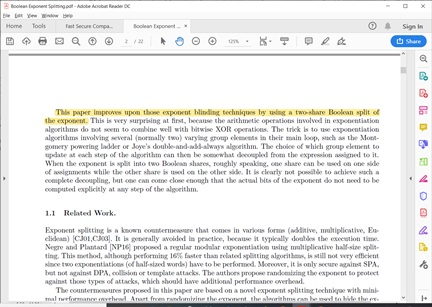
\includegraphics[scale=0.75]{Note1.jpg}
\caption{Note1: Highlighting a claim about a new countermeasure. \cite{tunstall2018boolean}}
\label{fig:Note1}
\end{figure}

\begin{figure}[ht!]
\centering
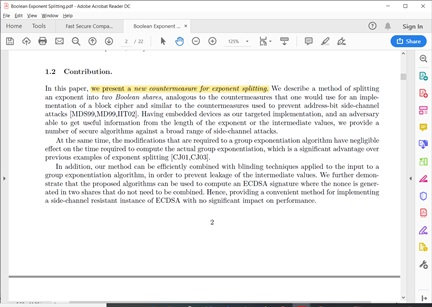
\includegraphics[scale=0.75]{Note2.jpg}
\caption{Note2: Highlighting a claim that technique improve state-of-the-art. \cite{tunstall2018boolean}}
\label{fig:Note2}
\end{figure}

\begin{figure}[ht!]
\centering
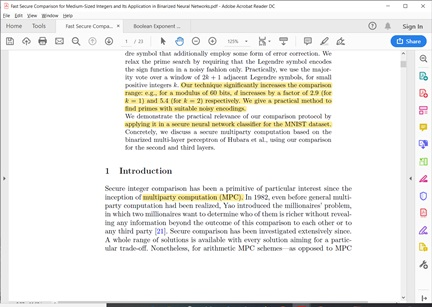
\includegraphics[scale=0.75]{Note3.jpg}
\caption{Note3: Highlighting a claim that technique improve state-of-the-art. \citep{abspoel2019fast}}
\label{fig:Note3}
\end{figure}

\section{Forced References}
I call this section forced references because I wanted all the "note= " that I put on the references be printed. The notes that I added are in \textbf{bold font} in the references. Maybe there is a better way of doing it on LaTex, but I do not know to do it that way as of now. Here are the papers that a read from the first paper on the list to the 60th papers published on the website of the International Association for Cryptologic Research (IACR) for 2018. https://www.iacr.org/  


\textbf{Papers that I critically read:} \cite{abspoel2019fast} \cite{tunstall2018boolean}



\textbf{Papers that I scanned}: \cite{patranabis2019function}
\cite{barreto2018qscms}
\cite{courtois2018structural}
\cite{baldimtsi2018universally}
\cite{abspoel2019fast}
\cite{tunstall2018boolean}
\cite{ghadafi2019further}
\cite{delcourt2018using}
\cite{deneuville2018cryptanalysis}
\cite{chatterjee2019large}

\textbf{Papers that I trashed}: \cite{ling2019accountable}
\cite{li2018two}
\cite{canetti2018fiat}
\cite{le2018senopra}
\cite{cheon2018multi}
\cite{canetti2018fully}
\cite{shishvan2018machine}
\cite{gazi2018proof}
\cite{yuan2018memory}
\cite{barak2019sum}
\cite{akavia2019setup}
\cite{zhao2018facct}
\cite{kandele2018key}
\cite{madala2018certificate}
\cite{abraham2018post}
\cite{lee2018pooled}
\cite{deng2018some}
\cite{cianciullo2018efficient}
\cite{wang2019xmss}
\cite{nilsson2019error}
\cite{chen2018implementing}
\cite{mizuide2019tight}
\cite{ashur2018cryptanalysis}
\cite{boneh2018exploring}
\cite{budaghyan2018changing}
\cite{kim2018new}
\cite{lee2018instant}
\cite{zotkin2018deep}
\cite{dinur2019multi}
\cite{lee2018countering}
\cite{dutta2019mprove}
\cite{liang2018teleportation}
\cite{xu2018revisiting}
\cite{sendrier2019decoding}
\cite{zhang2018arpa}
\cite{michalas2019lord}
\cite{banegas2019dags}
\cite{kim2018authcropper}
\cite{baek2019subversion}
\cite{renner2018rank}
\cite{galbraith2018quantum}
\cite{meyer2019lions}
\cite{belleville2018automated}
\cite{masure2019gradient}
\cite{de2019m}
\cite{beierle2018degree}
\cite{ito2019quantum}
\cite{kumar2018cryptanalysis}
\cite{chatterjee2019large}
 

%Testing note in citation \citep{patranabis2019function}
\bibliographystyle{plain}
\bibliographystyle{IEEEtran}
%\bibliography{references}
\bibliography{references2}
\end{document}
